% ====================================================================
%+
% SECTION:
%    MW_FutureWork.tex
%
% CHAPTER:
%    galaxy.tex
%
% ELEVATOR PITCH:
%    Ideas for future metric investigation, with quantitaive analysis
%    still pending.
%-
% ====================================================================

\section{Future Work}
\def\secname{MW_future}\label{sec:\secname}

% ====================================================================

% % ====================================================================
%+
% SECTION:
%    MW_Dust.tex
%
% CHAPTER:
%    galaxy.tex
%
% ELEVATOR PITCH:
%    Metric suggested - uncertainty and bias in $E(B-V)$~estimates as a
%    function of location on-sky - but not yet implemented.
%-
% ====================================================================

% \section{Dust in the Milky Way}
\subsection{Dust in the Milky Way}
\def\secname{MW_Dust}\label{sec:\secname}

\credit{pmmcgehee}
%,
%\credit{willclarkson}

As discussed in the LSST Science Book (particularly its Section 7.5),
possession of an accurate, three-dimensional dust map is important to
many astrophysical studies. The two most significant all-sky maps
generated in the past two decades are the SFD98 maps based on IRAS
observations, and the recent thermal dust maps derived from Planck
submillimeter data. The angular resolutions of both maps are similar -
between 4 to 6 arcminutes.

Both of the aforementioned maps are strictly two-dimensional and contain
no information about the distribution of dust along the line of sight. A
third dimension can be obtained by analysis of accurate stellar
photometry which constrains both the reddening $E(B-V)$ and extinction
$R_V \equiv A_V/E(B-V)$ towards individual stars. This approach requires
determination of the intrinsic stellar colors and the photometric
parallax of each star in the presence of an unknown amount and law of
extinction. Such maps are necessary to accurately measure the intrinsic
luminosities and colors of both Galactic and extragalactic sources.
Recent work on 3-D maps include the Bayesian analysis method based on
Pan-STARRS--1 (PS1) data \citep{green15} and an alternative technique
using SDSS photometry of M dwarfs (McGehee et al. 2016, in preparation).
However, these studies have so far typically been limited to
heliocentric distances of $\lesssim$4.5 kpc. In the full co-added
survey, LSST will be able to map dust structures out to distances
exceeding 40 kpc, thus revealing a detailed picture of this component of
the Milky Way Galaxy.

While the PS1 3-D dust map is a significant advance, it suggests a
number of major improvements that LSST will be able to
provide. Firstly, the PS1 map covers the region of the sky covered in
their 3$\pi$ survey, and thus excludes a large part of the Galactic
Plane towards the South. Secondly, the PS1 map \citep{2014ApJ...789...15S}
saturates at extinctions $E(B-V) > 1.5$ as their tracer stars fall out
of the survey catalogs fainter than $g\sim 22$, meaning that this
high-fidelity map does not extend uniformly to within a few degrees of
the midplane. Thirdly, this map is currently limited to distances $d
\lesssim 4.5$~kpc. Deep LSST data will allow this map to be extended
to much higher extinctions and larger distances. Owing to the high
extinction and the use of blue filters, this project is less affected
by crowding than other projects requiring photometry in the Plane.

The SDSS approach is complementary, and makes use of reddening-free
colors defined in the SDSS $ugriz$~system by \citet{mcgehee05}.
This approach makes use of M dwarf locus in $(g-r,r-i)$
being nearly perpendicular to the reddening vector in that color-color
space. This allows mapping of a reddening-invariant index to the
intrinsic stellar $g-i$ color and subsequent determination of the
light-of-sight reddening. This approach assumes a set extinction law,
i.e $R_V = 3.1$, in order compute the reddening-invariant index from
the observed $g-r$ and $r-i$ colors. Given the relative faintness of M
dwarfs, this technique is distance limited to $\sim$1 kpc when based
on SDSS data. With its significantly greater survey depth to M-dwarfs,
LSST should revolutionize the use of this technique to probe
Interstellar dust.

% --------------------------------------------------------------------

% \subsection{Target measurements and discoveries}
\subsubsection{Target measurements and discoveries}
\label{sec:\secname:targets}

LSST will be in a unique position to measure the changes in the
observed reddening vector due to $R_V$ variations due to its superb
photometric accuracy.  Both of the dust survey techniques mentioned
above can be used on LSST data, and perhaps other methods will be
developed before the start of survey operations.

When focusing on dust in the ISM (as
opposed to time-domain studies, e.g., dust around star-forming
regions or young stars), the main drivers of feasibility are
coverage of the few degrees around the Plane with sufficient photometric depth
and accuracy. This project is less affected by crowding than other
projects requiring photometry in the Plane owing to its use of blue
filters and the high extinction.  Nonetheless, quantiative estimates of
the expected photometric accuracy in coadded $u$ and $g$ images at low
Galactic latitude are desirable.

Production of a 3-D map of the dust component of the ISM based on LSST
photometry will tell us how much dust is present, what type it is, and
where it is along the line of sight.  The latter concern brings in
issues of how to determine stellar photometric parallaxes ($\mu = m-M$)
under an unknown reddening. The dust maps that are created will consist
of the median and variance of $E(B-V)$ and $R_V$ expressed as functions
of $\mu$ under a suitable binning scheme. We can create simple Figure of
Merit maps that lose the $\mu$ dependency by computing the mean and
variance of the measured variances in $E(B-V)$ and $R_V$ over the $\mu$
bins.

With the possible exception of sightlines towards star formation
regions, studies of interstellar dust are insensitive to the
distribution in time of the visits. In the case of active star formation
regions it is possible that changes in the ISM could be apparent over
the lifetime of the survey. Pushing to fainter magnitudes (which means
observing these fields with better seeing and longer exposures) will be
important, because more stars are required for better statistical
constraints on the model, because more stars are required that lie
behind the dust. In general, the use of broad band photometry requires
attention to the intrinsic SEDs of the background stars in order to
correct for heterochromatic variations in the effective reddening law.

% % --------------------------------------------------------------------
%
% \subsection{Metrics}
% \label{sec:\secname:metrics}
%
% {\bf Metric 1: Uncertainty and bias in $E(B-V)$~estimates as a
%   function of location on-sky.} Dependencies:
%
% \begin{itemize}
%   \item Stellar population throughout the survey %(e.g. Knut / Peter developments; TRILEGAL?);
%   \item Dust map throughout the survey region;
%   \item Scale photometric error predictions for each band from program requirements per exposure;
%   \item Produce formal estimate on the error in extinction and reddening as a function of position on-sky within the survey.
% \end{itemize}
%
%
% % --------------------------------------------------------------------
%
% \subsection{OpSim Analysis}
% \label{sec:\secname:analysis}
%
% Table \ref{tab_SummaryMWDust} summarizes the science Figures of Merit
% for the ISM science cases with LSST.
% % At the present date (April
% % 2016) placeholder rows are given for the FoM's.
%
% \begin{table}
%   \begin{tabular}{l|p{6cm}|c|c|c|c|p{5cm}}
%     FoM & Brief description & {\rotatebox{90}{\opsimdbref{db:baseCadence}}} & {\rotatebox{90}{\opsimdbref{db:opstwoPS}}} & {\rotatebox{90}{\scriptsize{\tt astro\_lsst\_01\_1004} }} &  {\rotatebox{90}{future run 2}} & Notes \\
%     \hline
%     1.1 & \footnotesize{Median (over sight-lines) of the uncertainty in $E(B-V)$} & - & - & - & - & \footnotesize{(Most useful FoM probably a spatial map of the uncertainty.)} \\
%     1.2 & \footnotesize{Variance (over sight-lines) of the uncertainty in $E(B-V)$} & - & - & - & - & - \\
%   \end{tabular}
% \caption{Summary of figures-of-merit for ISM science cases. The best
% value of each FoM is indicated in bold. Runs \opsimdbref{db:baseCadence}
% and \opsimdbref{db:opstwoPS} refer to the Baseline and PanSTARRS-like
% strategies, respectively. Column {\tt astro\_lsst\_01\_1004} refers to a
% recently-completed OpSim run that includes the Plane in Wide-Fast-Deep
% observations. See Section \ref{sec:MW_Disk}. }
% \label{tab_SummaryMWDust}
% \end{table}
%
%
% --------------------------------------------------------------------

%\subsection{Discussion}
%\label{sec:\secname:discussion}

%Discussion: what risks have been identified? What suggestions could be
%made to improve this science project's figure of merit, and mitigate
%the identified risks?

% ====================================================================
%
% \subsection{Conclusions}
%
% Here we answer the ten questions posed in
% \autoref{sec:intro:evaluation:caseConclusions}:
%
% \begin{description}
%
% \item[Q1:] {\it Does the science case place any constraints on the
% tradeoff between the sky coverage and coadded depth? For example, should
% the sky coverage be maximized (to $\sim$30,000 deg$^2$, as e.g., in
% Pan-STARRS) or the number of detected galaxies (the current baseline 
% of 18,000 deg$^2$)?}
%
% \item[A1:] ...
%
% \item[Q2:] {\it Does the science case place any constraints on the
% tradeoff between uniformity of sampling and frequency of  sampling? For
% example, a rolling cadence can provide enhanced sample rates over a part
% of the survey or the entire survey for a designated time at the cost of
% reduced sample rate the rest of the time (while maintaining the nominal
% total visit counts).}
%
% \item[A2:] ...
%
% \item[Q3:] {\it Does the science case place any constraints on the
% tradeoff between the single-visit depth and the number of visits
% (especially in the $u$-band where longer exposures would minimize the
% impact of the readout noise)?}
%
% \item[A3:] ...
%
% \item[Q4:] {\it Does the science case place any constraints on the
% Galactic plane coverage (spatial coverage, temporal sampling, visits per
% band)?}
%
% \item[A4:] ...
%
% \item[Q5:] {\it Does the science case place any constraints on the
% fraction of observing time allocated to each band?}
%
% \item[A5:] ...
%
% \item[Q6:] {\it Does the science case place any constraints on the
% cadence for deep drilling fields?}
%
% \item[A6:] ...
%
% \item[Q7:] {\it Assuming two visits per night, would the science case
% benefit if they are obtained in the same band or not?}
%
% \item[A7:] ...
%
% \item[Q8:] {\it Will the case science benefit from a special cadence
% prescription during commissioning or early in the survey, such as:
% acquiring a full 10-year count of visits for a small area (either in all
% the bands or in a  selected set); a greatly enhanced cadence for a small
% area?}
%
% \item[A8:] ...
%
% \item[Q9:] {\it Does the science case place any constraints on the
% sampling of observing conditions (e.g., seeing, dark sky, airmass),
% possibly as a function of band, etc.?}
%
% \item[A9:] ...
%
% \item[Q10:] {\it Does the case have science drivers that would require
% real-time exposure time optimization to obtain nearly constant
% single-visit limiting depth?}
%
% \item[A10:] ...
%
% \end{description}

% ====================================================================

\navigationbar


% ====================================================================

% WIC - promoted this back to MW Halo section

% % ====================================================================
%+
% SECTION:
%    MW_Halo.tex
%
% CHAPTER:
%    galaxy.tex
%
% ELEVATOR PITCH:
%
%-
% ====================================================================

\section{Mapping the Milky Way Halo}
%\subsection{Mapping the Milky Way Halo}
\def\secname{MW_Halo}\label{sec:\secname}

\credit{akvivas}, \credit{ctslater}, \credit{dnidever}

The study of the halo of the Milky Way is of the highest importance,
not only to understand the formation and early evolution of our own
galaxy, but also to test current models of hierarchical galaxy
formation. LSST will provide an unprecedented combination of area,
depth, wavelength range and long time-baseline for imaging data,
allowing detailed studies of the present-day structure of this old
Galactic component.  Here we
focus our attention on halo investigations using three tracer
populations. While we anticipate more cases will be developed and
compared between strategy choices, we have selected populations here
that illustrate many of the most important challenges.
%We focus here on three investigations of the Halo to be
%pursued with LSST data.
We describe the figures of merit (and the
diagnostic metrics on which they depend) that will allow quantitative
assessment of the impact of the choice of observing strategy on the
constraints LSST will afford.
%We expect more projects will join later.  % WIC - not sure what this meant.
We first briefly discuss the use of three main population tracers to
chart the halo population. More detail on each of these tracer
populations, and the general scientific motivations for studies of the
Milky Way halo with LSST, can be found in \citet{2009arXiv0912.0201L}.

{\it 1. RR Lyrae stars} have been known for several decades as
excellent tracers of the halo population. They are not only old stars
($>10$ Gyrs) but they are also excellent standard candles that allow
construction of three-dimensional maps. RR Lyrae stars have been used
to survey Milky Way halo populations extending out to
%The halo of the Milky Way has
%been now surveyed in a very large extension up to
$\sim 60-80$ kpc from the Galactic center \citep[][among
  others]{drake13a,drake13b,zinn14,torrealba15}. Beyond $\sim 80$~kpc,
the halo is mostly uncharted territory.

The RR Lyrae surveys suggest the halo is filled with substructures
(clumps of elevated stellar density) which are usually interpreted as
debris from destroyed satellite galaxies. This substructure overlies a
smooth component in the distribution of RR Lyrae stars, whose number density is well-described by a power law in galactocentric distance,
%which is well described
%with a power-law in the mean number density of RR Lyrae stars as a
%function of galactocentric distance,
steepening at radii $\gtrsim 30$ kpc \citep{zinn14}.  Thus, beyond
$\sim 60$ kpc, few field RR Lyrae stars are expected. However, we
presume that any RR Lyrae star beyond this distance may be part of
either debris material or distant low-luminosity satellite galaxies
% of low luminosity
that have been escaped detection until now \citep{sesar14,baker15}.
LCDM models predict debris as far as $0.5$~Mpc from the galactic
center. This is the territory that will be explored by LSST.

{\it 2. Red giant stars} can similarly be used to trace the structure
of the halo up to large distances. They have the advantage of being
bright and are numerous compared to the RR Lyrae stars but not as good
distance indicators.

{\it 3. Main sequence stars}, although less luminous than RR Lyraes or
Red Giants, are so much more numerous that statistical studies can be
pursued in a manner not generally possible for those populations.
%Fainter than these two tracers, main
%sequence stars stand up as a tool for studying the Halo. They are the
%most numerous type of stars available and statistical studies are
%possible.
Using the technique of photometric metallicities \citep{ivezic08}, the
Sloan Digital Sky Survey (SDSS) provided unprecedented maps of the
metallicity distribution up to $\sim 10$ kpc from the Galactic center,
unveiling not only the mean metallicity distribution of the halo but
also, sub-structures within the halo. LSST will extend these studies
all the way to the outermost parts of the Galaxy.
%This kind of works will be extended to the outermost parts of the
%Galaxy with LSST data.

% --------------------------------------------------------------------

\subsection{Target measurements and discoveries}
%\subsubsection{Target measurements and discoveries}
\label{sec:\secname:MW_Halo_targets}

Accurate measurement of these three tracer populations implies the following requirements:

%The three projects just described require the discovery and/or measurement of t%he following
%type of objects:

\begin{itemize}

\item[1.] RR Lyrae stars: These are bright horizontal-branch variable
  stars with periods between 0.2 to 1.0 days and large amplitudes,
  particularly in the bluer bandpasses (g amplitudes $0.5 -
  1.5$~mag). \citet{2012AJ....144....9O} made an intensive search for
  RR Lyrae stars in simulated LSST data and reached to the conclusion
  that this type of stars can be recovered to distances $\sim 600$
  kpc. A similar procedure can now be performed using MAF to directly
  compare LSST cadence scenarios to each other.
  %and current cadence scenarios.
  Chapter \ref{chp:variables} discusses the
  discovery metrics for variable stars including RR Lyrae
  stars. However, optimal recovery may involve more complex metrics
  involving the simultaneous use of multi-band time series
  \citep{vanderplas15,vivas16}. Besides recovery of variable stars,
  red-wavelength mean magnitudes $z$~and $y$ are particularly
  valuable since they provide the most accurate distance indicators.
  %valuable measurement to track for studies in the halo is the
  %infrared mean magnitudes z and y
\citep{caceres08}.

\item[2.] Main sequence stars: lacking any distinguishable variability, the
challenge in selecting a large and clean sample of main sequence stars comes
from tremendous number of small and nearly-unresolved galaxies present at
faint magnitudes. Precise star/galaxy separation is thus the limiting factor
on the useful depth of the main sequence sample. In addition to identifying
dwarfs, using dwarfs to map the metallicity distribution of the halo requires
precise $u$-band data, since it exhibits the strongest metallicity dependence of
the LSST filters.

\item[3.] Red Giants: due to their intrinsic luminosity, the Red Giants will sample
a far larger volume than main sequence stars at similar apparent magnitudes. However, they must first be identified and separated from the very numerous main
sequence stars present in the foreground. A gravity-sensitive photometric index can
be used for separating efficiently giants from dwarfs. The $u$-band magnitude is essential for such an index, so
%is
%an essential ingredient in this process, and
the behavior of the $u$-band limiting magnitude must therefore be charted under the various observational strategies under consideration.
% and it is necessary to follow-up
%the behavior of the u limiting magnitude under different observational
%strategies.
\autoref{fig-MW-giants} shows the distance that can be reached
by M-giants of different metallicities assuming limiting magnitude $u = 26.0$.
%-band limiting magnitude of 26.0..

\end{itemize}

\begin{figure}[h]
\begin{center}
  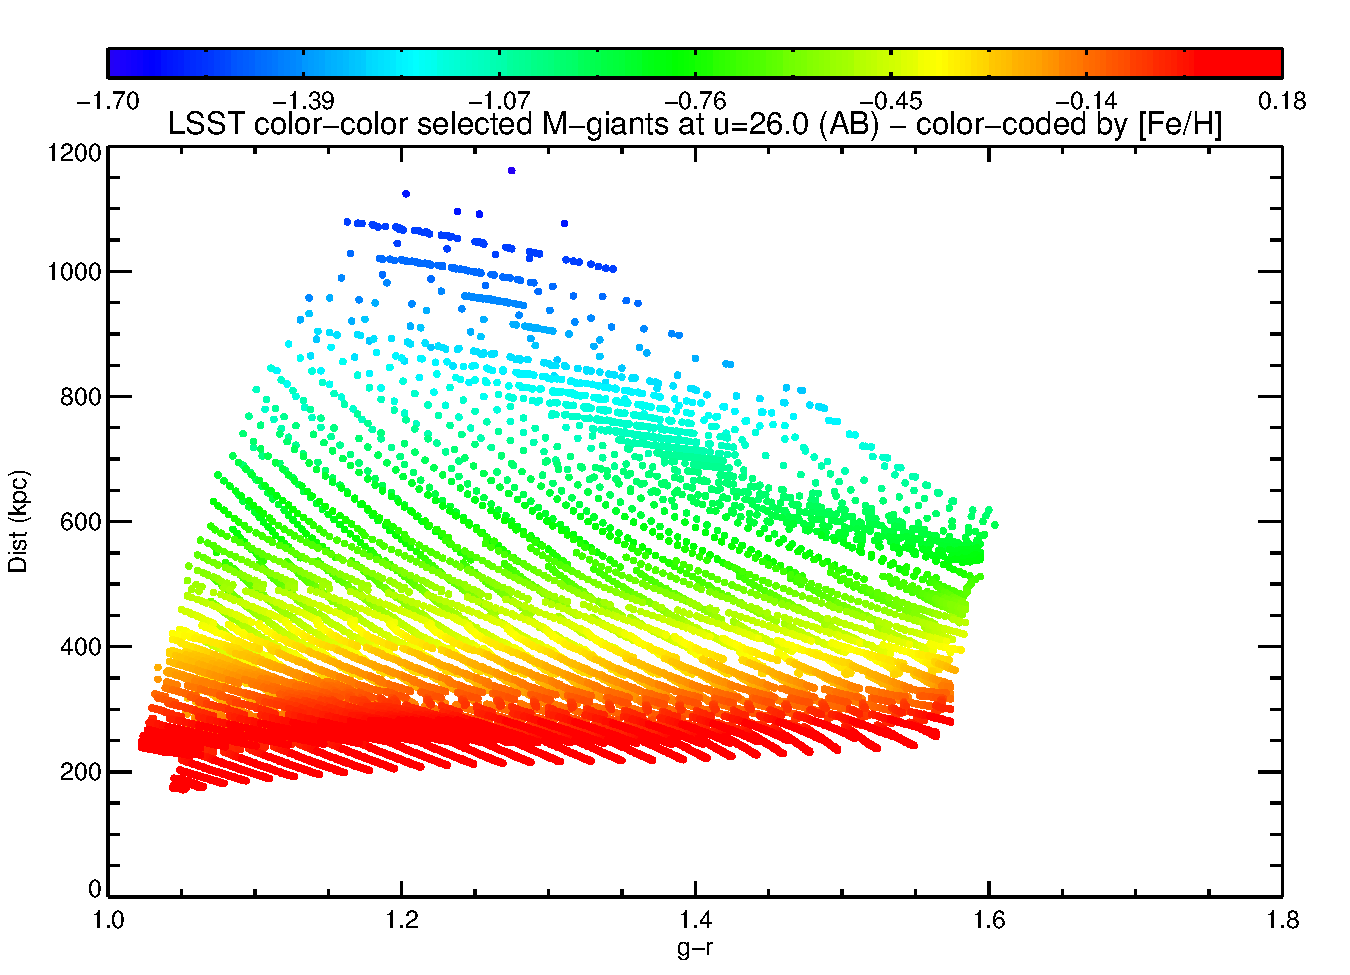
\includegraphics[scale=0.5]{./figs/milkyway/lsst_mgiants_grdist.pdf}
  \caption{Distance to which red giant stars can be identified in the galactic halo assuming a limiting magnitude
  of u=26.0. The color code scales with the metallicity of the stars. More metal-poor stars can be
  detected to farther distances. \label{fig-MW-giants}}
\end{center}
\end{figure}


% --------------------------------------------------------------------

\subsection{Metrics}
% \subsubsection{Metrics}
\label{sec:\secname:MW_Halo_metrics}

\textbf{Star-Galaxy Separation:} For main sequence stars, the useful depth of
the survey will likely not be the photometric detection limit, but will instead
be set by the ability to differentiate stars from unresolved background
galaxies. Towards faint magnitudes the contamination by galaxies worsens
significantly for several reasons: the number of galaxies is rising
substantially, the angular size of galaxies is shrinking, and our ability to
distinguish stars from marginally resolved galaxies diminishes for faint
sources simply due to photon statistics. While the fundamental properties of
the contaminant sources are beyond our control, our ability to reject these
sources depends on survey parameters which do vary with the choice of observing strategy, such as the distribution of seeing across
visits and the depth of these visits.

We are currently in the process of developing a metric that will estimate our
ability to separate stars and galaxies for any observation depth and seeing
conditions. This requires both an understanding of how images of a source are
measured and classified as either a star or galaxy, and how the population of
stars and galaxies vary in number and size (for galaxies) with depth. Our model
uses the distribution of galaxies in size and number, derived from HST COSMOS
observations, along with a fully Bayesian model decision formalism to compute
the expected completeness and contamination in star-galaxy separation.
Computationally, for each position in the survey footprint we interpolate the
results from that work on a grid in seeing, galaxy size, and coadd depth, then
integrate over the distribution of galaxy sizes. This modeling process is
currently being verified against existing surveys, and will be incorporated into
the observing strategy study at a later date.

%This is a diagnostic metric and some of the higher level metrics
%described below will depend on it.
Some of the higher-level figures of merit described below will depend on this star/galaxy separation diagnostic metric.

\textbf{Distance to the farthest RR Lyrae stars:} This metric charts our ability to
recover an RR Lyrae star from LSST data as a function of its distance. An RR Lyrae star may be
considered as recovered if its period and amplitude are within 10\% of the intrinsic values.
The procedure followed by \citet{2012AJ....144....9O} is a good example on how this can be
achieved. They built a large number of synthetic light curves spanning the properties of
known RR Lyrae stars and ``observed'' them with the cadence given by the \OpSim runs
available at that time. Anticipated improvements over this previous work include the use
of simultaneous multi-band information to recover periods \citep[e.g.,][]{vanderplas15,vivas16}.

However, a first look into this problem using MAF can be achieved
by simplifying the procedure and only test if a star with period 0.55 days (the mean period for
RR Lyrae stars) can be recovered by metrics already available in MAF.
Then, distance can be calculated using the mean magnitude of the recovered RR Lyrae stars
(in the reddest bands available to LSST) and the interstellar extinction at that point of the sky (maps are available
now in MAF).  This metric should compute the largest distance that can be measured with a 10\% precision
at which certain percentage of RR
Lyrae stars (eg. 80\%) can be recovered by LSST. It is expected that the results
of this metric at low galactic latitudes will be largely dependent on the chosen observational
strategy (through variations in cadence towards the Plane).
%(how sparse will the cadence be  in the galactic plane).

A reasonable Figure of Merit for this sub-project is the volume of the
halo within RR Lyrae stars  can be recovered. Similarly, another Figure
of Merit would be the fraction of the Galactic thick disk's volume that
can be traced by RR Lyrae stars.

\textbf{Distance to the farthest main sequence stars and giant stars:}
Since variability is not the signal property for these tracer
populations, metrics are somewhat simpler than for the RR Lyrae.
%Being non-variable objects,
%the metrics for these objects are somewhat simpler than for the RR Lyrae. and
Here the distance metric requires the determination of the limiting $u$-band
magnitude
%(in u band)
for which galaxy/star separation is reliable to a certain level. In
these cases, distances depend on metallicity. Then, a figure of merit is
the volume of the halo mapped with stars within a specified metallicity
range.

\textbf{WFIRST Synergy:} The extended optical-IR baseline that will be
provided by WFIRST \citep{2015arXiv150303757S} in $\sim 2,000$ sq degrees of the sky at high galactic latitudes
will provide additional ways to improve both the star-galaxy separation \citep[e.g.][]{banerji15} and the disentangling of stellar tracers in the halo
of the Milky Way \citep[e.g.][]{dalcanton12}. Chapter~\ref{chp:wfirst} discusses some areas of interaction between both
surveys. Metrics related to stellar populations in the halo using the overlap between both surveys are 
still to be developed.

% % --------------------------------------------------------------------
%
% \subsection{OpSim Analysis}
% \label{sec:\secname:MW_Halo_analysis}
%
% \autoref{tab_SummaryMWHalo} summarizes the science Figures of Merit
% for the Milky Way halo science cases for LSST.
% %OpSim analysis for this
% %Section will be summarized in that Table;
% At the present date (April
% 2016) placeholder rows are given for the FoM's. We welcome input from readers.
% %Input from the readers
% %is welcome!
%
% %%% SUMMARY TABLE FOR THIS SUBSECTION
%
% \begin{table}
%   \begin{tabular}{l|p{6cm}|c|c|c|c|p{5cm}}
%     FoM & Brief description & {\rotatebox{90}{\opsimdbref{db:baseCadence} }} & {\rotatebox{90}{\opsimdbref{db:opstwoPS} }} & {\rotatebox{90}{\scriptsize{\tt astro\_lsst\_01\_1004}  }} &  {\rotatebox{90}{future run 2}} & Notes \\
%     \hline
%     1.1. & \footnotesize{Survey volume to RR Lyraes}      & - & - & - & - & \footnotesize{Volume within which the distance to a template RR Lyrae star can be estimated to 10\% uncertainty.} \\
%     1.2. & \footnotesize{Survey volume to Main Sequence tracers} & - & - & - & - & \footnotesize{(Including star-galaxy separation)} \\
%     1.3. & \footnotesize{Survey volume to Red Giants} & - & - & - & - & - \\
% %    2.1. & \footnotesize{Completeness of metallicity sub-structure recovery as a function of distance} & - & - & - & - & \footnotesize{Over all three tracer populations?} \\
% %    3.1. & \footnotesize{Uncertainty and bias in age distribution parameterization of the main Halo population} & - & - & - & - & - \\
% %    3.2. & \footnotesize{Uncertainty and bias in the population fraction identified correctly with each halo component} & - & - & - & - & \footnotesize{Some overlap with Halo astrometry FoM?} \\
% \end{tabular}
% \caption{Summary of figures-of-merit (FoMs) for the Galactic Halo science cases. The best value of each FoM is indicated in bold. Runs \opsimdbref{db:baseCadence} and \opsimdbref{db:opstwoPS} refer to the Baseline and PanSTARRS-like strategies, respectively. Column {\tt astro\_lsst\_01\_1004} refers to a recently-completed OpSim run that includes the Plane in Wide-Fast-Deep observations. See Section \ref{sec:MW_Halo}.}
% \label{tab_SummaryMWHalo}
% \end{table}
%
%
% --------------------------------------------------------------------

%\subsection{Discussion}
%\label{sec:\secname:MW_Halo_discussion}

%Discussion: what risks have been identified? What suggestions could be
%made to improve this science project's figure of merit, and mitigate
%the identified risks?

% ====================================================================
%
\subsection{Conclusions}

 Here we answer the ten questions posed in
 \autoref{sec:intro:evaluation:caseConclusions}:

 \begin{description}

 \item[Q1:] {\it Does the science case place any constraints on the
 tradeoff between the sky coverage and coadded depth? For example, should
 the sky coverage be maximized (to $\sim$30,000 deg$^2$, as e.g., in
 Pan-STARRS) or the number of detected galaxies (the current baseline 
 of 18,000 deg$^2$)?}

\item[A1:] Yes - depth is generally preferred over increased
  sky-coverage. Fields with insufficient depth for star-galaxy
  separation to the required level of reliability will not be useful
  for the science in this section. While we expect this will lead to
  preference of achieving minimum depth vs expanding the sky-coverage,
  at this date we do not yet have quantitative limits.

 \item[Q2:] {\it Does the science case place any constraints on the
 tradeoff between uniformity of sampling and frequency of  sampling? For
 example, a rolling cadence can provide enhanced sample rates over a part
 of the survey or the entire survey for a designated time at the cost of
 reduced sample rate the rest of the time (while maintaining the nominal
 total visit counts).}

\item[A2:] Uniformity is generally preferred over sampling frequency. Coverage over the full ten-year survey must be maintained at sufficient cadence to be sensitive to RR Lyrae and $\delta$~Scuti populations, which are identified by variability. For the other tracers (where co-added depth is the key requirement), sampling considerations are less important.

 \item[Q3:] {\it Does the science case place any constraints on the
 tradeoff between the single-visit depth and the number of visits
 (especially in the $u$-band where longer exposures would minimize the
 impact of the readout noise)?}

\item[A3:] Single-visit depth is not a strong requirement for Halo science. Depth in $u$-band is dependent on the choice of tracer. For example, selection of red giants depends on accurate $u$-band photometry, which is not the case for turnoff stars (Section \ref{sec:MW_Halo:MW_Halo_targets}).

 \item[Q4:] {\it Does the science case place any constraints on the
 Galactic plane coverage (spatial coverage, temporal sampling, visits per
 band)?}

\item[A4:] No.

 \item[Q5:] {\it Does the science case place any constraints on the
 fraction of observing time allocated to each band?}

 \item[A5:] Yes, depending on the tracer population (Section \ref{sec:MW_Halo:MW_Halo_targets}).

 \item[Q6:] {\it Does the science case place any constraints on the
 cadence for deep drilling fields?}

\item[A6:] Not strongly. However, achieving huge co-added depth in fields containing Halo structure would greatly aid the understanding of observations of Halo structure throughout the main survey region.

 \item[Q7:] {\it Assuming two visits per night, would the science case
 benefit if they are obtained in the same band or not?}

\item[A7:] Halo science does not constrain the intra-night filter choice for a given field.

 \item[Q8:] {\it Will the case science benefit from a special cadence
 prescription during commissioning or early in the survey, such as:
 acquiring a full 10-year count of visits for a small area (either in all
 the bands or in a  selected set); a greatly enhanced cadence for a small
 area?}

\item[A8:] It would be good to observe at least a few fields towards known Halo structure, with a high fraction of observations in the first year or so, to best characterize LSST's performance for Halo science and make predictions for the rest of the survey.

 \item[Q9:] {\it Does the science case place any constraints on the
 sampling of observing conditions (e.g., seeing, dark sky, airmass),
 possibly as a function of band, etc.?}

\item[A9:] Generally best-seeing is preferred to enable star/galaxy separation. We do not at this date have quantitiative evaluations of a Figure of Merit for this, however.

 \item[Q10:] {\it Does the case have science drivers that would require
 real-time exposure time optimization to obtain nearly constant
 single-visit limiting depth?}

\item[A10:] No.

\end{description}

% ====================================================================

\navigationbar


% ====================================================================

% \subsection{Other Ideas}

\credit{willclarkson}, \credit{akvivas}, \credit{vpdebattista}

In this final section we provide an extremely brief list of important science
cases that are still in an early stage of development, but that are
deserving of quantitative \MAF analysis in the future.

\subsection{Further considerations for Milky Way static science}

  One important area of Milky Way science on which further
  community input is still sorely needed, is {\it static science} (a
  category that includes population disentanglement through deep,
  multicolor photometry), particularly in regions outside the main
  ``Wide-Fast-Deep'' (WFD) survey (Sections \ref{sec:MW_Astrometry} \&
  \ref{sec:MW_Halo} include discussion of static science in WFD regions). Since
  static science depends on depth (for, e.g., precise colors near the
  main sequence turn-off of some population) and uniformity over the
  survey (to aid characterization of strong selection functions),
  static science observing requirements may be in tension with (or at
  least not explicitly addressed by) requirements communicated
  elsewhere in this chapter.

  For example, probing deep within spatially crowded
  populations may lead to a sharper requirement on the selection of
  observations in good seeing conditions towards crowded regions, than
  has been apparent to-date. This needs quantification. 

  To pick another example, while we have indicated that co-added
  depth is a lower priority than temporal coverage for
  variability-driven studies in the Galactic Disk (conclusion A.1 in
  Section \ref{sec:MW_Disk}), co-added depth will likely be crucial for
  population disentanglement through photometry. While a
  judiciously-chosen observing strategy should be able to support both
  static and variable science, at this date quantitative trade-offs have not yet been specified.

  In many cases the implementation of figures of merit for static
  science in the Milky Way is complicated by the requirement to
  interface custom population simulations with the observational
  characterizations produced by the \MAF framework. For many
  investigators, the preferred method may be to use \MAF to produce
  parameterizations of the observational quantities of interest - for
  example, the run of photometric uncertainty against apparent
  magnitude, for each location on the sky, and including spatial
  confusion (all of which \MAF can currently produce\footnote{See the tutorials at \url{https://github.com/LSST-nonproject/sims_maf_contrib} for more information.}) - and then use
  these characteristics as input to their own population simulations,
  on which the investigator may have invested substantial time and
  effort.

  To provoke progress, we specify in Table
  \ref{table:strawmanMWstaticScience} a possible Figure of Merit for
  static science in terms of capabilities mostly already provided by
  the \MAF framework, which does not require custom simulation. This
  Figure of Merit - which asks what fraction of fields in a spatial
  region of interest, are sufficiently well-observed to permit
  population disentanglement to some desired level of precision -
  could form the basis of several science FoM's (for example, the
  fraction of fields in which photometric age determinations of
  bulge/bar populations might be attempted). We encourage community
  development and implementation of this and other FoMs for Milky Way
  static science.

\begin{table}[h]
  \small
  \begin{tabular}{c p{12cm}}
    & {\it FoM innerMW-Static: fraction of fields in inner Galactic plane adequately covered for population discrimination} \\
    \hline
    1. & Produce absolute magnitudes $M_{u,g,r,i,z,y}$~of the population of interest, using \MAF's spectral libraries; \\
    2. & For each HEALPIX (i.e. pointing):\\
       & 2.1. Place the fiducial star at appropriate line-of-sight distance, produce apparent magnitudes $m_{u,g,r,i,z,y}$;\\
       & 2.2. Modify $m_{u,g,r,i,z,y}$~for extinction using \MAF's extinction model;\\
    & 2.3. Compute the photometric and astrometric uncertainties due to sampling and random error (from \MAF's ``m52snr'' method);\\
    & 2.4. Convert exposure-by-exposure estimates of photometric and astrometric uncertainty due to spatial confusion, into co-added uncertainties;\\
    & 2.5. Combine the random and confusion uncertainties into final measurement uncertainties on the photometry and astrometry;\\
    & 2.6. Use uncertainty propagation to estimate color uncertainties $u-g, g-r, r-i, i-z$;\\
    3. & Count the fraction of sight-lines for which the color below the threshold needed for "sufficient" accuracy in parameter determination \citep{ivezic08}. {\bf This is the figure of merit.} \\
\hline
    \end{tabular}
 \caption{Description of Figure of merit ``innerMW-Static''}
  \label{table:strawmanMWstaticScience}
\end{table}

Finally, we provide an extremely brief list of important science
cases that are still in an early stage of development, which fall into the ``Static science'' category of Milky Way science:
\begin{itemize}
  \item {\it Formation history of the Bulge and present-day balance of
  populations:} Sensitivity to metallicity and age distribution of Bulge
  objects near the Main Sequence Turn-off;
  \item {\it Migration and heating in the Milky Way disk:} Error and
  bias in the determination of components in the (velocity dispersion vs
  metallicity) diagram, for disk populations along various lines of
  sight \citep[e.g.][]{2016ApJ...818L...6L}.

% WIC 2017-05-24: commented this out in favor of a dedicated local volume subsection.
%
%\item Fraction of Local-Volume objects discovered as a function of
%  survey strategy.
\end{itemize}

\subsection{Short exposures}

  Populations near, or brighter than, LSST's nominal saturation
  limit ($r \sim 16$~with 15s exposures) are likely to be crucial to a
  number of investigations for Milky Way investigations, whether as
  science tracers in their own right, or as contaminants that might
  interfere with measurements of fainter program objects (due, for
  example, to charge bleeds of bright, foreground disk objects).

  Quantitative exploration of these issues now requires involvement from
  the community (e.g. to determine LSST's discovery space for bright
  tracers in context with other facilities and surveys like ZTF, Gaia
  and VVV), and the project (e.g. to determine the parameters of short
  exposures that might be supported by the facility). To provoke
  development, here we list a few example questions regarding short
  exposures that still need resolution:

\begin{itemize}
  \item{What level of bright-object charge-bleeding can be tolerated? For example, is some minimum distribution of position-angles required in order to spread the bleeds azimuthally over the set of observations of a particular line of sight (so that different pixels fall under bleeds in different exposures)?\footnote{Note that with $\sim 30$~exposures per filter per field over ten years towards some regions, charge bleeds on the detector for a given object might not be spread over a large range of orientations. The spread of charge bleed angles on the detector - as a spatially-varying metric - should be implemented and included in figures of merit.} What is this minimum?}
    \item{What is the science impact of restricting targets to $r \gtrsim 16$?}
      \item{Will the proposed twilight survey of short exposures be adequate for science cases requiring short exposures? Are there enough observations from other surveys (e.g. DES or other DECam surveys) to cover the bright end of the entire LSST footprint, and are {\it new} observations of very bright objects required scientifically in any case?}
        \item{What is the bright limit required for adequate astrometric cross-calibration against Gaia?}
          \item{To what extent would a given bright cutoff hamper the combination of LSST photometry or astrometry with that from other surveys (like VVV)?}
          \item{How short an exposure time can the facility support? Does the OpSim framework already include all the operational limitations on scheduling short exposures?}
\end{itemize}


\subsection{The Local Volume}

  Finally, we remind the reader that substantial opportunity
  remains to develop science figures of merit for {\it Local Volume}
  science cases. Figures of Merit for Local Volume science likely
  share much common ground with those for the Halo (discussed in
  Section \ref{sec:MW_Halo}), and substantial prior expertise exists
  \citep[e.g.][]{2014ApJ...795L..13H}. One straightforward Figure of
  Merit (FoM) might be the fraction of dwarf galaxies in the Local
  Volume that are correctly identified as a function of survey
  strategy.

% ====================================================================

\navigationbar
